\section{Step 83 Finish the Up tail without overreading}
Fill \texttt{row\_up\_tail}. If the destination already equals the exclusive end, continue directly to row completion. Otherwise load one residual and one upper byte, add and store the low byte, advance both pointers, and repeat. Converge on \texttt{row\_up\_tail\_ready} once the entire remainder has been consumed. The supplied next label completes the row.

For up6, two bytes remain after the vector group. At the first tail checkpoint all eighteen samples of row zero are 250, and both cursors are at their sample-window ends. The next row becomes eighteen samples of value four. The complete call returns zero and 38 bytes: two rows, each containing one retained selector and eighteen reconstructed samples.

Repeat with widths one, five and seventeen. They give sample extents 3, 15 and 51, exposing a tail-only row, a boundary just below a vector, and three vectors followed by three bytes. Compare scalar and MSA outputs exactly. Counts and equal images are necessary, but the access checks must also establish that neither path reads a selector or the next row as spare vector lanes.

\paragraph{Observe} Use \texttt{s83-1}; stop before \texttt{row\_up\_tail\_ready}. Inspect the state described above before continuing.

\Needspace{7\baselineskip}
Figure~\ref{fig:png-row-reconstruction} stops at the first Up-tail checkpoint.
Count nineteen bytes per row: one selector and eighteen samples. The first row's
samples are all \texttt{fa}; the next row still contains \texttt{0a} residuals.
The remaining-row register is still two because row completion follows the
checkpoint. Do not treat that intermediate register as a completed return value.

% Native editable composition from verified, unchanged IDE images.
\begin{figure}[htbp]
\centering
\sbox0{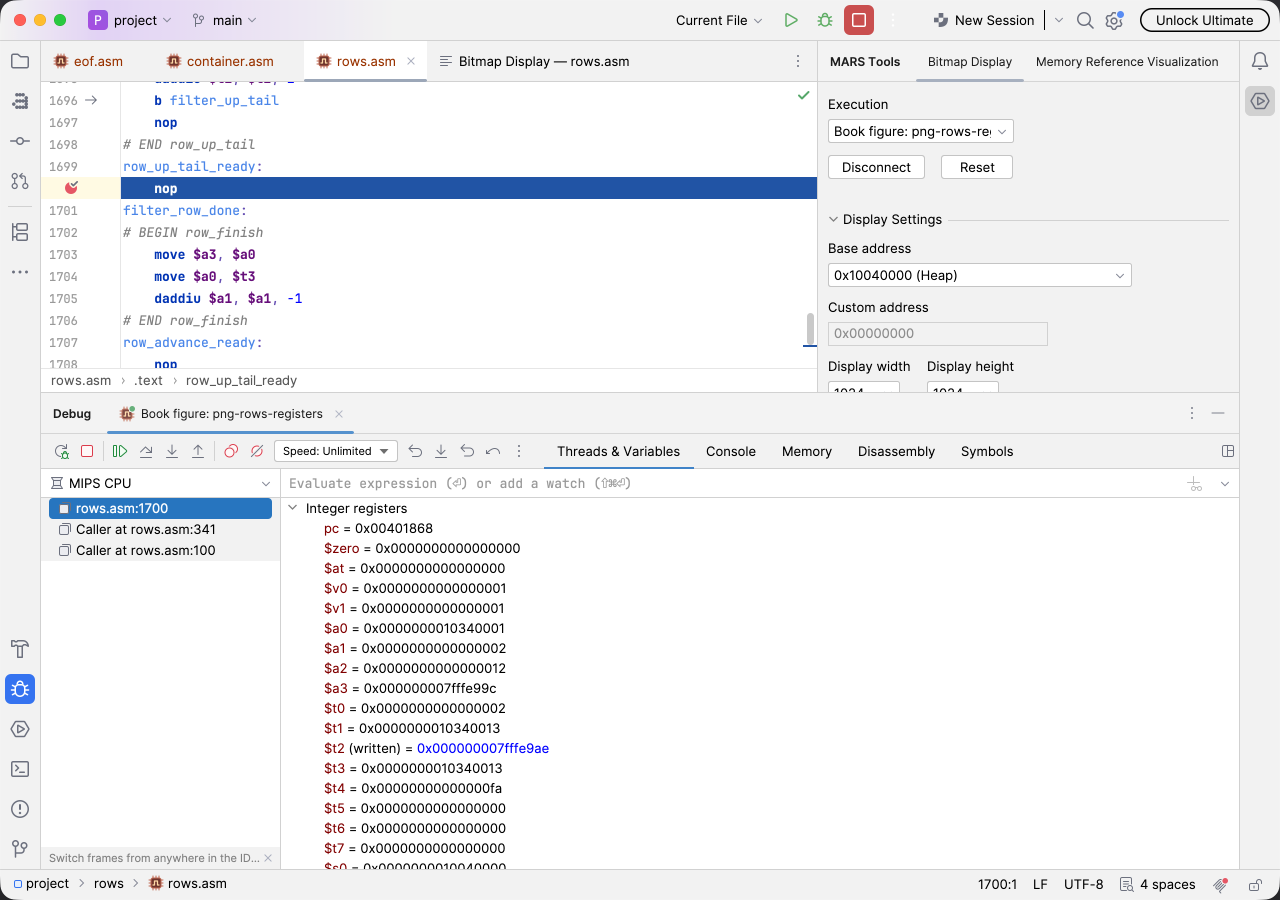
\includegraphics[artifact]{packages/033-png/captures/png-row-reconstruction/registers.png}}
\sbox2{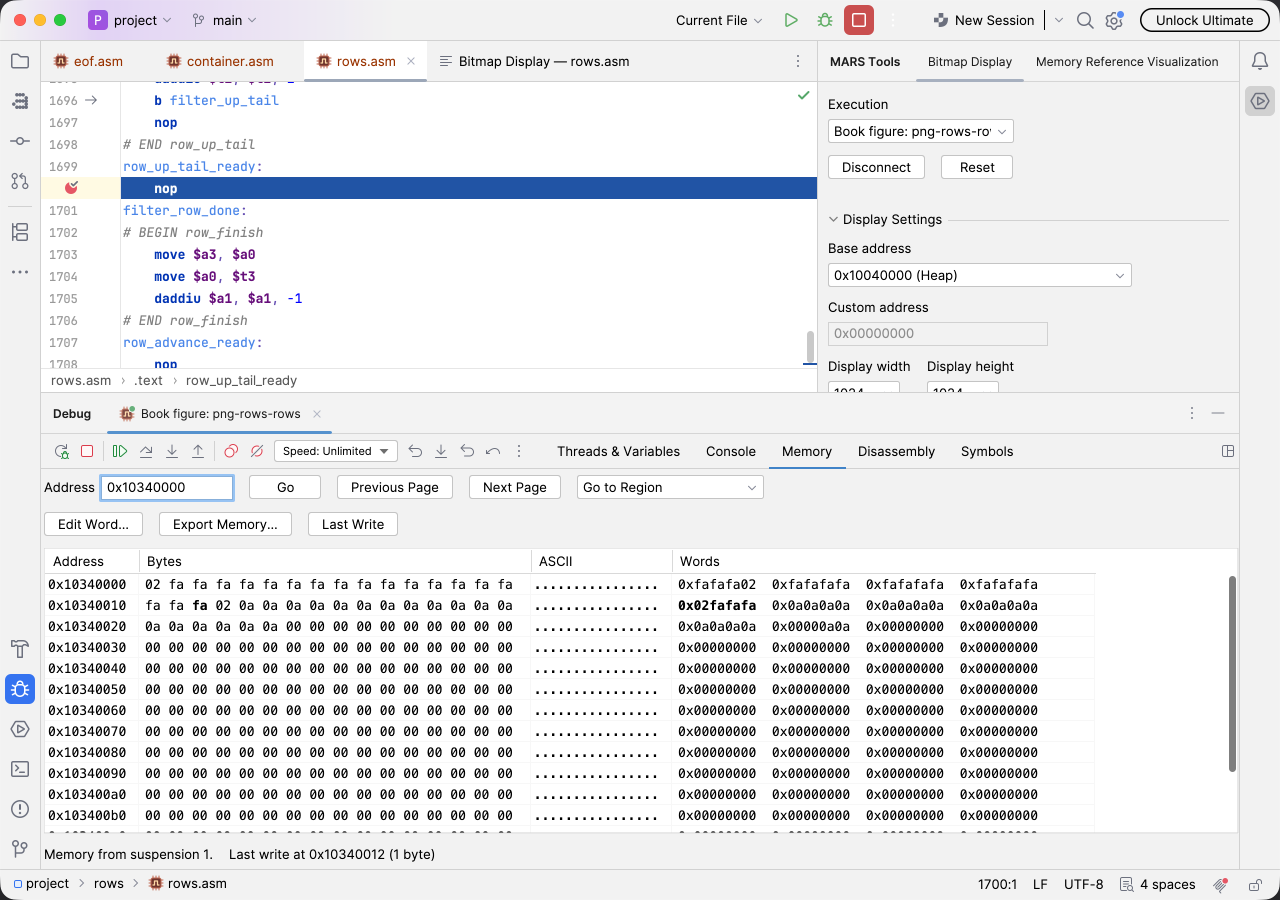
\includegraphics[artifact]{packages/033-png/captures/png-row-reconstruction/rows.png}}
\edef\MARSrowssourceLeft{\the\dimexpr0.036718750\wd0\relax}
\edef\MARSrowssourceBottom{\the\dimexpr0.774444444\ht0\relax}
\edef\MARSrowssourceRight{\the\dimexpr0.611718750\wd0\relax}
\edef\MARSrowssourceTop{\the\dimexpr0.170000000\ht0\relax}
\edef\MARSrowsrowsLeft{\the\dimexpr0.108593750\wd2\relax}
\edef\MARSrowsrowsBottom{\the\dimexpr0.288888889\ht2\relax}
\edef\MARSrowsrowsRight{\the\dimexpr0.585156250\wd2\relax}
\edef\MARSrowsrowsTop{\the\dimexpr0.634444444\ht2\relax}
\edef\MARSrowsremainingLeft{\the\dimexpr0.246093750\wd0\relax}
\edef\MARSrowsremainingBottom{\the\dimexpr0.265555556\ht0\relax}
\edef\MARSrowsremainingRight{\the\dimexpr0.598437500\wd0\relax}
\edef\MARSrowsremainingTop{\the\dimexpr0.705555556\ht0\relax}
\begin{tikzpicture}[alt={Three annotated IDE details at row_up_tail_ready before its nop. The first selector remains 02 followed by eighteen fa bytes, reconstructed samples of 250. Offset nineteen holds the next selector 02 followed by eighteen residual bytes 0a, which have not been reconstructed yet. Register a1 is two because the first row has not reached row completion.}]
\node[anchor=north west,inner sep=0,font=\small\bfseries] (source-title) at (6mm,0) {First Up-tail checkpoint};
\node[anchor=north west,inner sep=0] (source) at ([yshift=-1mm]source-title.south west) {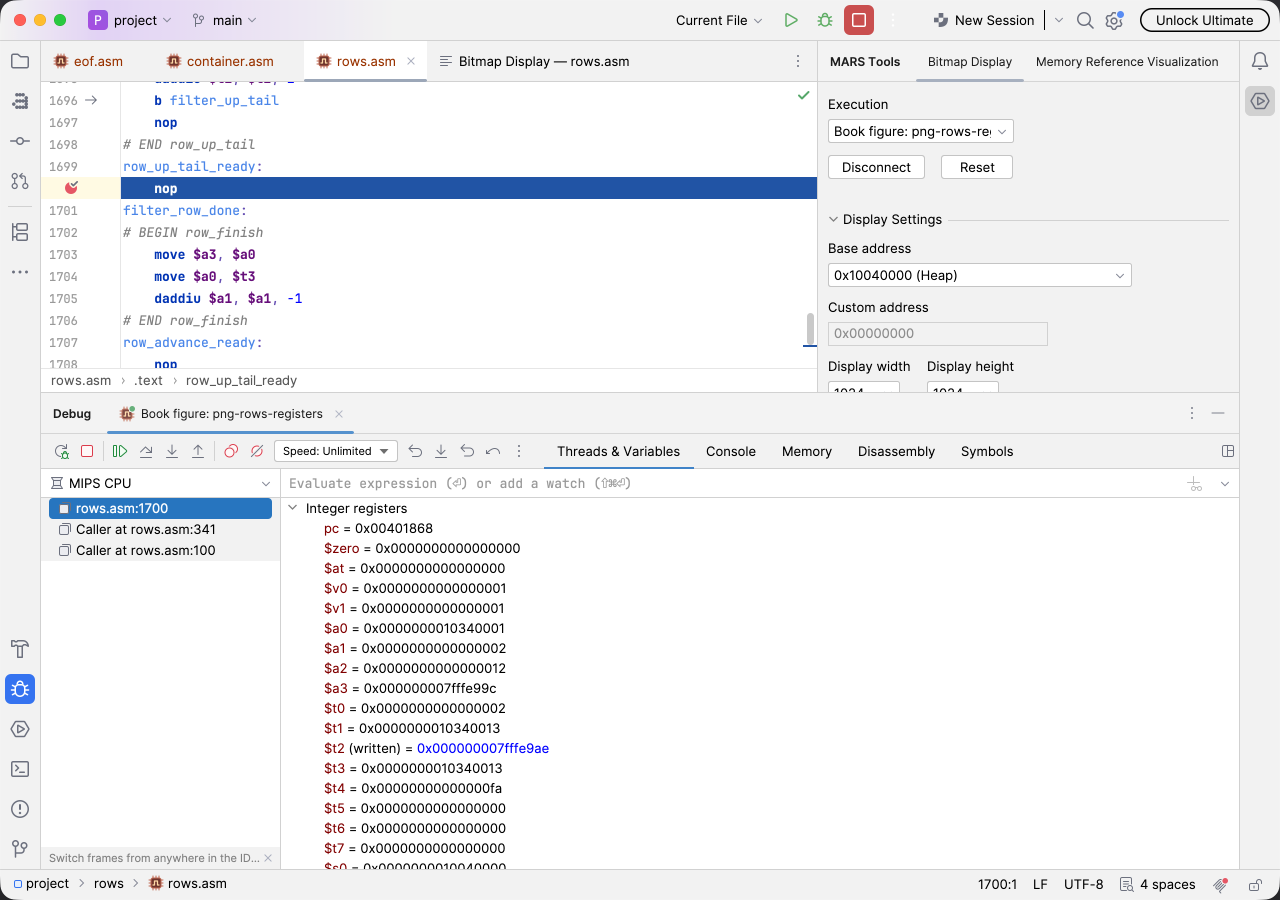
\includegraphics[width=0.7\linewidth,artifact,trim={\MARSrowssourceLeft{} \MARSrowssourceBottom{} \MARSrowssourceRight{} \MARSrowssourceTop{}},clip]{packages/033-png/captures/png-row-reconstruction/registers.png}};
\begin{scope}[shift={(source.south west)},x={($(source.south east)-(source.south west)$)},y={($(source.north west)-(source.south west)$)}]
\draw[black,line width=0.7pt] (0.168888889,0.080000000) rectangle (0.288888889,0.520000000);
\node[draw=black,fill=white,circle,inner sep=1.5pt,font=\footnotesize] at ($(0.168888889,0.520000000)+(-3mm,0)$) {1};
\end{scope}
\node[anchor=north west,inner sep=0,font=\small\bfseries] (rows-title) at ([yshift=-2mm]source.south west) {Retained selectors and reconstructed samples};
\node[anchor=north west,inner sep=0] (rows) at ([yshift=-1mm]rows-title.south west) {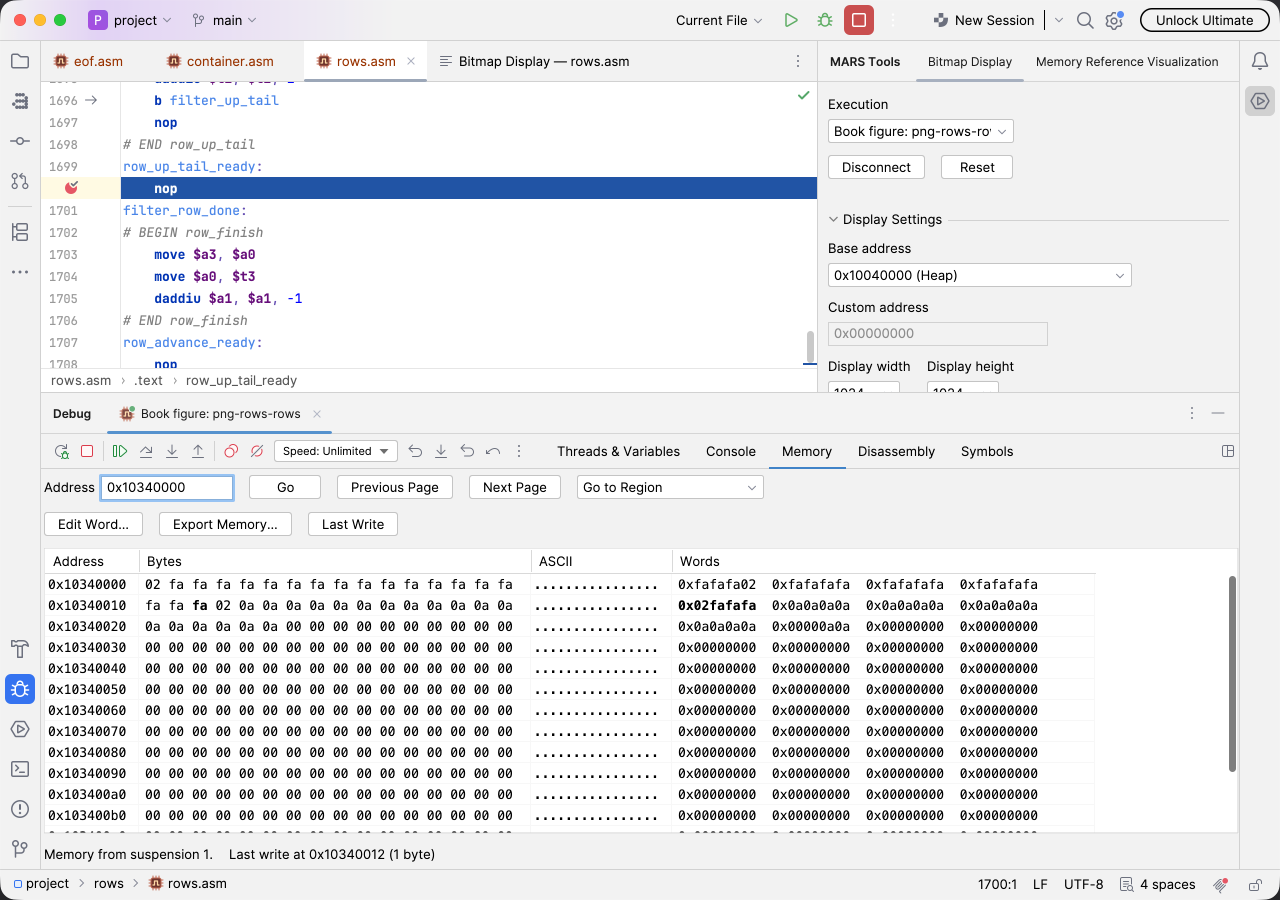
\includegraphics[width=0.84\linewidth,artifact,trim={\MARSrowsrowsLeft{} \MARSrowsrowsBottom{} \MARSrowsrowsRight{} \MARSrowsrowsTop{}},clip]{packages/033-png/captures/png-row-reconstruction/rows.png}};
\begin{scope}[shift={(rows.south west)},x={($(rows.south east)-(rows.south west)$)},y={($(rows.north west)-(rows.south west)$)}]
\draw[black,line width=0.7pt] (0.000000000,0.043478261) rectangle (1.000000000,0.956521739);
\node[draw=black,fill=white,circle,inner sep=1.5pt,font=\footnotesize] at ($(0.000000000,0.956521739)+(-3mm,0)$) {2};
\end{scope}
\node[anchor=north west,inner sep=0,font=\small\bfseries] (remaining-title) at ([yshift=-2mm]rows.south west) {Rows before the completion decrement};
\node[anchor=north west,inner sep=0] (remaining) at ([yshift=-1mm]remaining-title.south west) {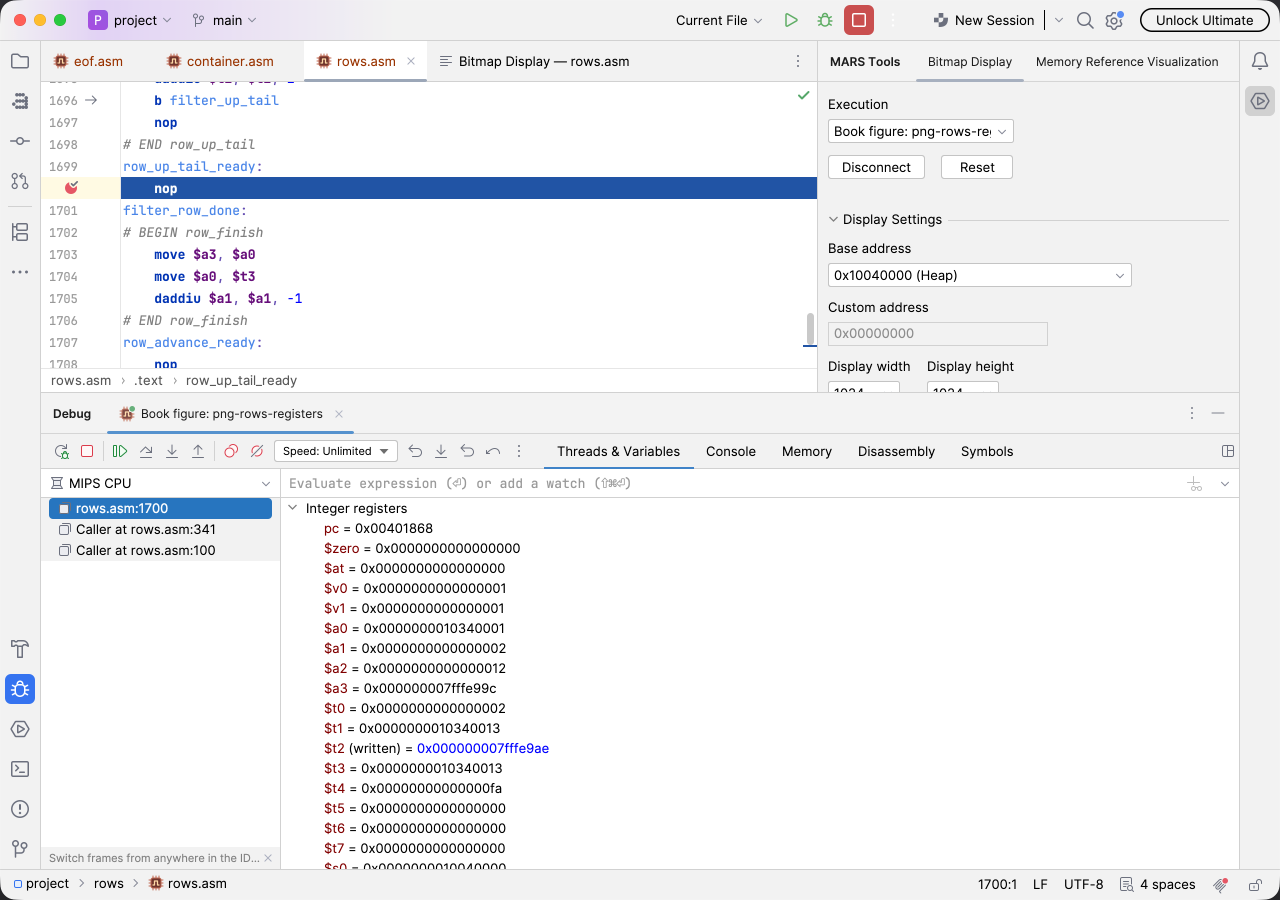
\includegraphics[width=0.5\linewidth,artifact,trim={\MARSrowsremainingLeft{} \MARSrowsremainingBottom{} \MARSrowsremainingRight{} \MARSrowsremainingTop{}},clip]{packages/033-png/captures/png-row-reconstruction/registers.png}};
\begin{scope}[shift={(remaining.south west)},x={($(remaining.south east)-(remaining.south west)$)},y={($(remaining.north west)-(remaining.south west)$)}]
\draw[black,line width=0.7pt] (0.030150754,0.115384615) rectangle (0.969849246,0.884615385);
\node[draw=black,fill=white,circle,inner sep=1.5pt,font=\footnotesize] at ($(0.030150754,0.884615385)+(-3mm,0)$) {3};
\end{scope}
\end{tikzpicture}
\par\smallskip
\begin{minipage}{\linewidth}
\small
\begin{enumerate}
\item The first row has consumed its sixteen-byte vector group and two-byte scalar tail. Both sample cursors are exactly at their exclusive ends.
\item The first 38 bytes are two 19-byte rows. Selector \texttt{02} is followed by eighteen \texttt{fa} samples in row zero. Row one still contains selector \texttt{02} and eighteen \texttt{0a} residuals; its later reconstruction produces \texttt{04}. The following zero bytes lie outside these rows.
\item \texttt{\$a1}=2 because \texttt{filter\_row\_done} has not decremented the remaining-row count. This intermediate register is specific to the illustrated implementation.
\end{enumerate}
\end{minipage}
\caption{The first Up-filtered row after its vector group and scalar tail. Two Debug launches stop at the same first-row boundary.}
\label{fig:png-row-reconstruction}
\end{figure}

\clearpage

\paragraph{Check} What must an empty Up tail do?
\begin{itemize}
  \item[A.] Load one vector to discover its length.
  \item[B.] Reach row completion without a sample load.
  \item[C.] Overwrite the selector with zero.
\end{itemize}
